%%% LaTeX Template: Article/Thesis/etc. with colored headings and special fonts
%%%
%%% Source: http://www.howtotex.com/
%%% Feel free to distribute this template, but please keep to referal to http://www.howtotex.com/ here.
%%% February 2011
%%%
%%% Modified January 2016 by CDM

%%%  Preamble
\documentclass[11pt,letterpaper]{article}
\usepackage[margin=1.0in]{geometry}
\usepackage[T1]{fontenc}
\usepackage[bitstream-charter]{mathdesign}
\usepackage[latin1]{inputenc}					
\usepackage{amsmath}						
\usepackage{xcolor}
\usepackage{cite}
\usepackage{hyphenat}
\usepackage{graphicx}
\usepackage{float}
\usepackage{subfigure}
\usepackage{sectsty}
\usepackage[compact]{titlesec} 
\usepackage[tablegrid]{vhistory}
\usepackage{pbox}
\allsectionsfont{\color{accentcolor}\scshape\selectfont}

%%% Definitions
\definecolor{accentcolor}{rgb}{0.0,0.0,0.5} 
\newcommand{\teamname}{Team Tassium}
\newcommand{\productname}{Master Chef}
\newcommand{\coursename}{CSE 4316: Senior Design I}
\newcommand{\semester}{Fall 2017}
\newcommand{\docname}{Architectural Design Specification}
\newcommand{\department}{Department of Computer Science \& Engineering}
\newcommand{\university}{The University of Texas at Arlington}
\newcommand{\authors}{Anthony Tatowicz \\ Jesse Daniel Mitchell \\ Todd Brewer\\ Linh Vu}

%%% Headers and footers
\usepackage{fancyhdr}
	\pagestyle{fancy}						% Enabling the custom headers/footers
\usepackage{lastpage}	
	% Header (empty)
	\lhead{}
	\chead{}
	\rhead{}
	% Footer
	\lfoot{\footnotesize \teamname \ - \semester}
	\cfoot{}
	\rfoot{\footnotesize page \thepage\ of \pageref{LastPage}}	% "Page 1 of 2"
	\renewcommand{\headrulewidth}{0.0pt}
	\renewcommand{\footrulewidth}{0.4pt}

%%% Change the abstract environment
\usepackage[runin]{abstract}			% runin option for a run-in title
%\setlength\absleftindent{30pt}			% left margin
%\setlength\absrightindent{30pt}		% right margin
\abslabeldelim{\quad}	
\setlength{\abstitleskip}{-10pt}
\renewcommand{\abstractname}{}
\renewcommand{\abstracttextfont}{\color{accentcolor} \small \slshape}	% slanted text

%%% Start of the document
\begin{document}

%%% Cover sheet
{\centering \huge \color{accentcolor} \sc \textbf{\department \\ \university} \par}
\vspace{1 in}
{\centering \huge \color{accentcolor} \sc \textbf{\docname \\ \coursename \\ \semester} \par}
\vspace{0.5 in}
\begin{figure}[h!]
	\centering
   	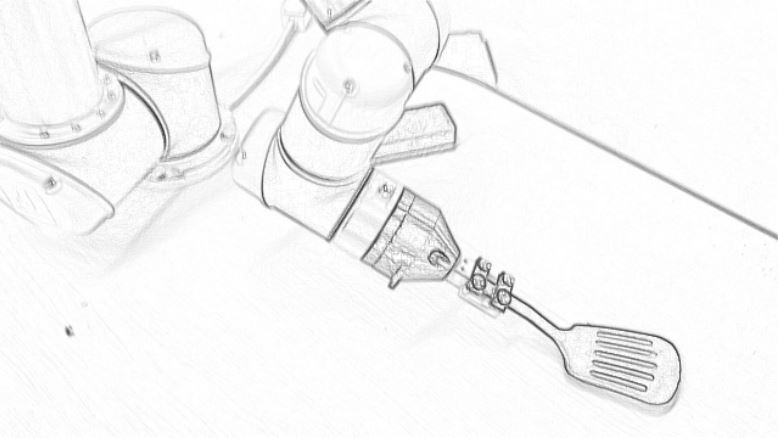
\includegraphics[width=0.60\textwidth]{images/test_image}
\end{figure}
\vspace{0.5 in}
{\centering \huge \color{accentcolor} \sc \textbf{\teamname \\ \productname} \par}
\vspace{0.5 in}
{\centering \large \sc \textbf{\authors} \par}
\newpage


%\vspace{1 in}
%\centerline{January 13th, 2012}
%\newpage

%%% Revision History
\begin{versionhistory}
  	\vhEntry{0.1}{12.04.2017}{LV, JDM}{First draft}
  	\vhEntry{0.1}{5.09.2018}{LV, TB}{Revise documents, add pictures}
\end{versionhistory}
\newpage

%%% Table of contents
\setcounter{tocdepth}{2}
\tableofcontents
\newpage

%%% List of figures and tables (optional)
\listoffigures
\listoftables
\newpage

%%% Document sections
\section{Introduction}
The UR5 Master Chef is a product that aims to alleviate the need for manual labor in a cooking environment.  The purpose of this design is to provide an interchangeable tool interface allowing for the use of various tools for use in a fast paced food preparation area. The target application for his prototype is to demonstrate the creation, preparation, and serving of grill cheese sandwiches.
\newpage
\section{System Overview}
The main architecture of the system involves 4 main systems communicating with each other. The control logic system and UR5 system pass information with each other via the network system through an Ethernet TCP/IP connection.  The UR5 then provides a signal to the mount system allowing for the docking and undocking of various utensils.

\begin{figure}[h!]
	\centering
 	\includegraphics[width=0.60\textwidth]{images/ADS_layers}
 \caption{A simple architectural layer diagram}
\end{figure}

\subsection{Network}
%%%Each layer should be described separately in detail. Descriptions should include the features, functions, critical interfaces %%%and interactions of the layer. The description should clearly define the services that the layer provides. Also include any %%%%conventions that your team will use in describing the structure: naming conventions for layers, subsystems, modules, and data %%%flows; interface specifications; how layers and subsystems are defined; etc.
This layer contains the router that will allow a connection to the UR5.

\subsection{Control}
This layer contains the camera, raspberry pi that will be use to communicate with the UR5.

\subsection{Mount}
This layer contains the mount that will fit the tool into the mount by controlling the magnet.

\subsection{UR5}
This layer contains the UR5 robot arm, the polyscope(interface), and the control box.
\newpage
\section{Subsystem Definitions \& Data Flow}
This section breaks down your layer abstraction to another level of detail. Here you grapically represent the logical subsytems that compose each layer and show the interactions/interfaces between those subsystems. A subsystem can be thought of as a programming unit that implements one of the major functions of the layer. It, therefore, has data elements that serve as source/sinks for other subsystems. The logical data elements that flow between subsystems need to be explicitly defined at this point, beginning with a data flow-like diagram based on the block diagram.

\begin{figure}[h!]
	\centering
 	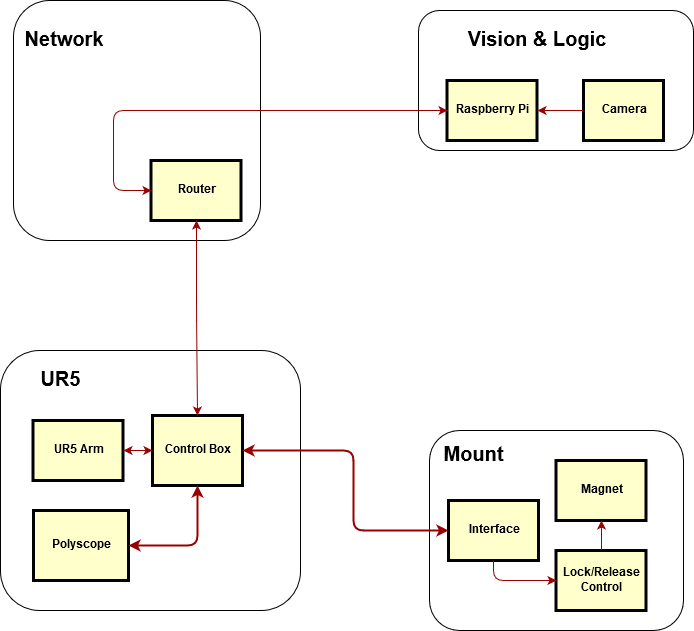
\includegraphics[width=\textwidth]{images/ADS_data_flow}
 \caption{A simple data flow diagram}
\end{figure}

\newpage
\section{Network Layer Subsystems}
This layer is for communication between the control layer and the UR5 layer in details. It have a router as its subsystem. The router uses DHCP to allow IP addresses to be assigned to the UR5's control box and the Raspberry Pi.

\subsection{Network Layer Hardware}
N/A

\subsection{Network Layer Operating System}
N/A

\subsection{Netowrk Layer Software Dependencies}
Requires TCP/IP socket connection method in software.

\subsection{Router}
Router is the only piece of hardware in the Network Layer. It requires Ethernet cables to be connected to the UR5 control box and Raspberry Pi  establish  TCP/IP socket connection for issuing commands to the UR5's robotic arm.

\begin{figure}[h!]
	\centering
 	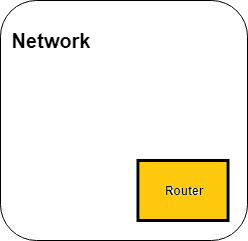
\includegraphics[width=0.60\textwidth]{images/Network_Layer_Router}
 \caption{Router Subsystem diagram}
\end{figure}

\subsubsection{Router Subsystem Hardware}
Standard wired Ethernet router.

\subsubsection{Router Subsystem Operating System}
N/A

\subsubsection{Router Subsystem Software Dependencies}
Requires TCP/IP socket connection method in software.

\subsubsection{Router Subsystem Programming Languages}
N/A

\subsubsection{Router Subsystem Data Structures}
Structure of commands issued from Raspberry Pi to UR5 are sent as strings converted to bytes. For example the string 'stop(1.0)' would be converted to bytes and sent to the robot to tell it to stop.

\subsubsection{Router Subsystem Data Processing}
N/A



\newpage
\section{Control Layer Subsystems}
This layer is the integration of the UI and camera in details.

\begin{figure}[h!]
	\centering
 	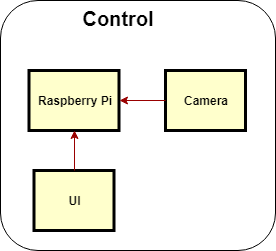
\includegraphics[width=0.60\textwidth]{images/Control_Layer}
 \caption{Control layer diagram}
\end{figure}

\subsection{User Interface}
The user interface operate through a browser that allow the user to give specifics task to the UR5.

\subsubsection{Assumptions}
The browser the user will be using is google chrome. Other browser may works just as well, this project however, has been operating the UI through google chrome.

\subsubsection{Responsibilities}
The purpose of this UI is to allow the user to gives specific command to the UR5. The commands are as follow::
	Home  		: Move UR5 to default position.
	Start 		: Make grill cheese sandwich.
	Stop  		: Cease function.
	Rack Tool 	: Put away tool.
	Grab Tool 	: Grab tool.
	
*The tools for this project specifically is a spatula. Other tools will be implement later in the future.

\subsubsection{Subsystem Interfaces}
The UI connects to the raspberry pi.

\begin {table}[H]
\caption {UI interfaces} 
\begin{center}
    \begin{tabular}{ | p{1cm} | p{6cm} | p{3cm} | p{3cm} |}
    \hline
    ID & Description & Inputs & Outputs \\ \hline
    \#xx & Rasberry Pi & \pbox{3cm}{N/A} & \pbox{3cm}{UI \\ Commands}  \\ \hline
    \end{tabular}
\end{center}
\end{table}

\subsection{Camera}
The camera use to determine the location of certain object(sandwich) or if there is another object in the way of the UR5.

\subsubsection{Assumptions}
The camera is a 720p or higher.
At least one camera.

\subsubsection{Responsibilities}
The purpose of the camera is to determine the location of the sandwich relative to its position so that the UR5 can pick up the sandwich. Its other responsibility is also to detect foreign obstacle or human being so that it can stop before colliding.

\subsubsection{Subsystem Interfaces}
The camera connects to the raspberry pi.

\begin {table}[H]
\caption {Camera interfaces} 
\begin{center}
    \begin{tabular}{ | p{1cm} | p{6cm} | p{3cm} | p{3cm} |}
    \hline
    ID & Description & Inputs & Outputs \\ \hline
    \#xx & Rasberry Pi & \pbox{3cm}{N/A} & \pbox{3cm}{Location of sandwich\\ Detect foreign obstacle or human being}  \\ \hline
    \end{tabular}
\end{center}
\end{table}

\subsection{Raspberry Pi}

\subsubsection{Assumptions}

\subsubsection{Responsibilities}

\subsubsection{Subsystem Interfaces}

\begin {table}[H]
\caption {Raspberry Pi interfaces} 
\begin{center}
    \begin{tabular}{ | p{1cm} | p{6cm} | p{3cm} | p{3cm} |}
    \hline
    ID & Description & Inputs & Outputs \\ \hline
    \#xx & UI & \pbox{3cm}{N/A} & \pbox{3cm}{N/A}  \\ \hline
    \#xx & Camera & \pbox{3cm}{N/A} & \pbox{3cm}{N/A}  \\ \hline
    \end{tabular}
\end{center}
\end{table}


\newpage
\section{UR5 Layer Subsystems}
This layer is the destination of all the instructions from the control layer go to. It contains the UR5's arm, its control box, and a polyscope for the UI.

\begin{figure}[h!]
	\centering
 	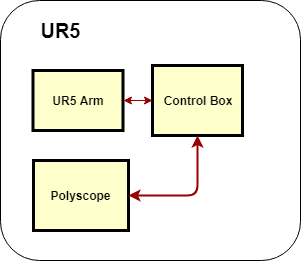
\includegraphics[width=0.60\textwidth]{images/UR5_Layer}
 \caption{UR5 layer diagram}
\end{figure}

\subsection{UR5 Arm}
This is the physical arm of the UR5. It receives instruction from the control box and act accordingly.

\subsubsection{Assumptions}
The arm is fully functional and can pick up at least 5 pounds.
It is connected to the control box.
It comes with the control box and polyscope.

\subsubsection{Responsibilities}
This arm takes in instruction from the UI. It moves accordingly to what the user instructions through the UI.


\subsubsection{Subsystem Interfaces}
The arm is connected to the control box as its interface.

\begin {table}[H]
\caption {UR5 Arm interfaces} 
\begin{center}
    \begin{tabular}{ | p{1cm} | p{6cm} | p{3cm} | p{3cm} |}
    \hline
    ID & Description & Inputs & Outputs \\ \hline
    \#xx & UR5 control box & \pbox{3cm}{Instructions(UR script)} & \pbox{3cm}{Position of arm}  \\ \hline
    \end{tabular}
\end{center}
\end{table}

\subsection{Control Box}
The control box is what allow the arm to receive instructions and move accordingly. It receives instruction from the UI through the polyscope or it can receive instructions from an outside source through a socket.

\subsubsection{Assumptions}
Functional and connects to the arm.
It comes with the arm and polyscope.

\subsubsection{Responsibilities}
The control box receive inputs and then outputs the instruction to the arm.

\subsubsection{Subsystem Interfaces}
The control box is connected to the arm and the polyscope. It is also controlling the connector that is on the wrist of the arm.

\begin {table}[H]
\caption {Control Box interfaces} 
\begin{center}
    \begin{tabular}{ | p{1cm} | p{6cm} | p{3cm} | p{3cm} |}
    \hline
    ID & Description & Inputs & Outputs \\ \hline
    \#xx & UR5 Arm & \pbox{3cm}{Position of Arm} & \pbox{3cm}{Waypoints \\ UR scripts}  \\ \hline
    \#xx & Polyscope & \pbox{3cm}{Instructions(UR script) \\ Waypoints \\ I/O control \\ Voltage} & \pbox{3cm}{Position of arm \\ I/O control\\ Voltage}  \\ \hline
    \#xx & Connector & \pbox{3cm}{N/A} & \pbox{3cm}{Voltage}  \\ \hline
    \end{tabular}
\end{center}
\end{table}

\subsection{Polyscope}
The polyscope is a UI that comes with the UR5. It is where all the script and control of the UR5 movements that can be instructed by writing a script.

\subsubsection{Assumptions}
The user is not using the polyscope as a way of sending the the instructions to the arm.
It is connected to the control box.
It comes with the control box and the arm.

\subsubsection{Responsibilities}
The emergency stop button is use to stop the arm immediately.

\subsubsection{Subsystem Interfaces}
The polyscope interface is the control box.

\begin {table}[H]
\caption {Polyscope interfaces} 
\begin{center}
    \begin{tabular}{ | p{1cm} | p{6cm} | p{3cm} | p{3cm} |}
    \hline
    ID & Description & Inputs & Outputs \\ \hline
    \#xx & UR5 control box & \pbox{3cm}{Position of arm \\ I/O control\\ Voltage} & \pbox{3cm}{Instructions(UR script) \\ Waypoints \\ I/O control \\ Voltage}  \\ \hline
    \end{tabular}
\end{center}
\end{table}


\newpage
\section{Mount Layer Subsystems}
This layer is the mount that control the release and hold of the tool.

\begin{figure}[h!]
	\centering
 	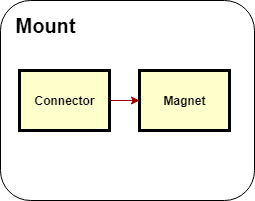
\includegraphics[width=0.60\textwidth]{images/Mount_Layer}
 \caption{Mount layer diagram}
\end{figure}

\subsection{Connector}
The connector is mounted on the wrist of the arm, but it is being control by the control box.

\subsubsection{Assumptions}
There is a 8 pin connector at the wrist of the arm and an available Lumberg RKMV 8-354 cable for the 8-pin connector.

\subsubsection{Responsibilities}
This connector control the mount to grab or release the tool by sending the magnet either 12v or 0v respectively.

\subsubsection{Subsystem Interfaces}
The connector interacts with the magnet by the instructions of the control box.

\begin {table}[H]
\caption {Connector interfaces} 
\begin{center}
    \begin{tabular}{ | p{1cm} | p{6cm} | p{3cm} | p{3cm} |}
    \hline
    ID & Description & Inputs & Outputs \\ \hline
    \#xx & Control Box & \pbox{3cm}{Voltage(0v or 12v)} & \pbox{3cm}{N/A}  \\ \hline
    \#xx & Magnet & \pbox{3cm}{N/A} & \pbox{3cm}{Voltage(0v or 12v}  \\ \hline
    \end{tabular}
\end{center}
\end{table}

\subsection{Magnet}
The magnet is place inside the mount where the tool can be inserted.

\subsubsection{Assumptions}
The magnet is strong enough to hold at least 5 pounds.
It receives either 0v or 12v from the UR5.
It does not takes more than 12v.

\subsubsection{Responsibilities}
The magnet is to grab/hold or release the tool by receiving either 0v or 12v.

\subsubsection{Subsystem Interfaces}
The magnet interface with the connector.

\begin {table}[H]
\caption {Magnet interfaces} 
\begin{center}
    \begin{tabular}{ | p{1cm} | p{6cm} | p{3cm} | p{3cm} |}
    \hline
    ID & Description & Inputs & Outputs \\ \hline
    \#xx & Connector & \pbox{3cm}{Voltage(0v or 12v)} & \pbox{3cm}{N/A}  \\ \hline
    \end{tabular}
\end{center}
\end{table}



\newpage

%%% References
\bibliographystyle{plain}
\bibliographystyle{reference/IEEEtran_custom}
\bibliography{reference/refs}{}

\end{document}